%------------------------------------------------------
%Author             : Jonathan Schwarz
%University         : Pforzheim University
%Date of last edit  : Fri, 06 Mar 2015 10:00:53 +0100
%Filename           : neural_networks.tex
%------------------------------------------------------

\documentclass[10pt,a4paper,DIV=11]{scrreprt}

%British English
\usepackage[UKenglish]{babel}
\usepackage[tbtags]{amsmath}
%utf8
\usepackage[utf8]{inputenc}

%pseudo-code
\usepackage[boxruled,vlined]{algorithm2e}

\usepackage{scrhack}
%for source code listings
\usepackage{listings}

\usepackage[table]{xcolor}

%tikz
\usepackage{tikz}
\usetikzlibrary{arrows, positioning, fit}


%male and female symbol
\usepackage{wasysym}
%plots
\usepackage{pgfplots}

%blocks - used by tikz-uml, included before
\pgfdeclarelayer{background}
\pgfdeclarelayer{foreground}
\pgfsetlayers{background,main,foreground}

%<,> in tikz-uml
\usepackage[T1]{fontenc}
% \usepackage{tikz-uml}

%subfigure
\usepackage{graphicx}
\usepackage{subfigure}

%prevent figure from floating pictures
%\usepackage{float}

%footer & header
\usepackage{fancyhdr}

%push footer down
\usepackage[bottom]{footmisc}

%footer & header
\pagestyle{fancy}
%clean footer & header
\fancyhf{}

%acronyms
\usepackage[nohyperlinks]{acronym}

%bibtex
\usepackage[square,numbers]{natbib}
\usepackage{gensymb}

%maths
\usepackage{amssymb} 
\usepackage{dsfont}

%japanese
\usepackage{CJKutf8}

%table of contents with hyperlinks
%always include as last package
\usepackage{hyperref}

%===========================TITLE PAGE=======================================

%university logo
\titlehead
{
    
\includegraphics[width=0.20\textwidth]{files/hspflogo.pdf}\\

    Pforzheim University\\
    School of Engineering\\
}

\subject{Project work}
	
\title
{
     A comparison of neural network types and learning techniques with an application in artificial life.
}

\author
{
    \textbf{Jonathan Schwarz} - matriculation number: 304727
}
\date
{
    Summer term 2015
}
%\today{}}

\publishers
{
    Examiner: Prof. Dr. Richard Alznauer\\
    Supervisor: Dr. Christoph Ußfeller
}


%=========================================GLOBAL SETTINGS=========================================

%footer &header

%\fancyfoot[L]{\textbf{Multi-Threading mit POSIX-pThreads}}
\fancyhead[R]{Page \thepage}
%\fancyhead[L]{\thechapter}

%chapter number and title
\fancyhead[L]{\nouppercase{\leftmark}}
%line
%\renewcommand{\footrulewidth}{0.5 pt}
\usepackage{lmodern}
\addtokomafont{sectioning}{\rmfamily}
\setlength{\parindent}{0mm}

%colour definitions
\definecolor{dkgreen}{rgb}{0,0.6,0}
\definecolor{grey}{rgb}{0.7,0.7,0.7}
%medium grey
\definecolor{mgrey}{gray}{0.80}
%light grey
\definecolor{lgrey}{gray}{0.97}

%hyperlink settings
%frame around hyperlinks
\hypersetup
{
    colorlinks = false,
    linkcolor = black,
    hypertexnames = false,
    citecolor = green
}

%listing settings
\lstset
{ 
    language=C,                
    basicstyle=\footnotesize\ttfamily,           
    numbers=left,
    stepnumber=5,    
    firstnumber=1,
    numberfirstline=true                 
    numberstyle=\color{black},                 
    numbersep=5pt,                 
    backgroundcolor=\color{white},      
    showspaces=false,             
    showstringspaces=false,         
    showtabs=false,                
    frame=single,                   
    rulecolor=\color{black},       
    tabsize=2,                     
    captionpos=b,                   
    breaklines=true,                
    breakatwhitespace=false,       
    title=\lstname,                    
    keywordstyle=\color{blue},          
    commentstyle=\color{dkgreen}, 
    identifierstyle=\color{black},      
    stringstyle=\color{purple},      
    escapeinside={\%*}{*)},      
    morekeywords={*,...},            
    deletekeywords={...}             
}

\newenvironment{Japanese}{%
    \CJKfamily{min}%
    \CJKtilde
\CJKnospace}{}

\setcounter{tocdepth}{4}  %a deeper contents menue
%=====================================DOCUMENT START=========================
\begin{document}

\tikzstyle{line}=[draw]
\tikzstyle{arrow}=[draw, -latex] 

%\renewcommand*\contentsname{Content}
%\renewcommand*\listtablename{Tables}
%\renewcommand*\listfigurename{Figures}
%\renewcommand*\bibname{Literature references}

\maketitle
\thispagestyle{empty}
\newpage
{\large\tableofcontents}
\newpage

\thispagestyle{empty}

\section*{List of acronyms}
\begin{acronym}
    \acro{$ANN$}{Artificial neural network}
    \acro{$a_j$}{Activity of unit $n_j$}
    \acro{$a_j(t)$}{Activity of unit $n_j$ at time $t$}
    \acro{$H$}{The set of hidden layers of a neural network}
    \acro{$L$}{The set of layers of a neural network}
    \acro{$ML$}{Machine learning}
    \acro{$MLN$}{Multi layer network}
    \acro{$n_j$}{Neuron (also unit) $j$}
    \acro{$W$}{The connection matrix}
    \acro{$w_{ij}$}{Weight on the connection link between neurons $n_i$ and $n_j$}
%    \acro{$\Delta w_{ij}$}{Weight change  on the connection link between unit $i$ and $j$}
%    \acro{$\overrightarrow{x}$}{The input vector of a neural network}
%    \acro{$\overrightarrow{y}$}{The output vector of a neural network}
%    \acro{$\varphi$}{Activation (transfer) function of a neuron}
%    \acro{$\eta$}{Learning rate of a network}
%    \acro{$\nabla F(a)$}{Gradient of the multivariable function $F(x)$ at point $a$}
\end{acronym}

\newpage

\chapter{Introduction}
In \cite{DANIEL}, Schembri proposes the application of machine learning algorithms for training of object collecting agents. 
Such agents dwell in a simulated, confined, two-dimensional space, where objects are dropped at random. Without any previous knowledge of 
their environment, agents are placed in the world and are to reason that their aim is to collect objects. The performance or fitness of each 
individual is rated by the amount of objects collected in a given time period. Thus, this fitness ranking serves as a quality measure for the 
chosen approaches.

In particular, Schembri is interested in using artificial neural networks to devise a control policy for each agent at any point in time. 
Unsupervised learning with genetic algorithms is chosen as the means to achieve satisfactory behaviour. Its principle is to alter 
an agents behaviour and evaluate whether this amendment improved or lowered the agents performance. In case of a successful change, the changes
will be accepted, whereas they are reverted if the change was not. By gradual application of this technique, Schembri tries to increase
the performance so as to achieve intelligent behaviour.
This project builds off of Schembri's work and both extends the unsupervised approach and also shows that successful learning can be 
achieved by means of previous training. The basic rationale behind this supervised approach is that an agent is presented a set of correct 
policies from given input to output data. It is then to learn from this given data and mimic the underlying control policy and apply it to
previously unseen data. In addition to the learning approach, alterations in the neural network structure can also have significant influence
to the agents performance. Hence, different structures will be proposed and empirically evaluated.

Both approaches will be tested in the very same simulation environment as in the original paper. A critical evaluation of both learning approaches
in combination with different network structures is given.

\paragraph{Structure of this project}
%TODO: Really exposed?
In chapter \ref{ch:basics} a brief introduction to the very basics of artificial neural networks is given. We investigate their biological counterpart
and show a mathematical formalisation of their structure. We dive more into the details of artificial neural networks in chapter \ref{ch:ANN} where
we talk about different models and network structure. Different learning algorithms are presented in chapter \label{ch:learning}. We show both
supervised and unsupervised algorithms and expose their limitations. The application and evaluation of presented algorithms is shown in
chapter \label{ch:eval}, where we critically analyse the performance gain in comparison to Schembri's work. A final conclusion is drawn in 
\label{ch:conclusion} and further ideas of how to improve the performance are given in chapter \label{ch:future}.

\chapter{Basics}
\label{ch:basics}
\section{Neural networks}
The operation of artificial neural networks (ANNs) is based on and modeled after the understanding of the human brain. 
Our brain is an astonishingly powerful information processing system. It is capable of solving extremely complex tasks such as recognising a face, or
processing vision and audio signals simultaneously at ease. In contrast, programming a computer to do so turns out to be rather difficult.
A distinctive feature is their ability to learn and abstract from examples. As distinct from computers, ANNs do not have to be programmed to solve 
a certain task. This feature makes them particularly interesting for tasks where no solution or at least no efficient algorithm
exist. Further examples of successful applications of neural networks are given in section \ref{sec:exp}.
In terms of computability ANNs are an equivalent model to the Turing machine.\cite{NURING}

Neural networks may be looked at from widely different angles. Their models serve neuroscience for the understanding of biological processes 
in the human brain, while a psychologist verifies learning- and memory theories using those models. A physicist regards them as a physical structure,
which can be described by their energy functions and probabilistic regularities. From a computer scientific point of view, neural networks
are massive parallelized, adaptive and partially self-organised information processing systems. \cite{NNGER}
Within this project, neural network (or rather artificial ones) are regarded as a machine learning algorithm. 
Machine learning itself may be understood as a sub field or means to an end of artificial intelligence.
We are particularly interested in using them to define a decision policy for intelligent agents. Such a decision policy uses knowledge of the agent's
environment, obtained by sensors, to manipulate it using its actuators. This is done in a way to maximise the expected future reward (collecting as
many objects as possible). Nevertheless, a brief explanation of their biological inspiration promotes the understanding of their structure and is 
therefore given in the following sections. In addition, we show how they have been described mathematically, which allows their representation 
in a computer program.

\section{Biological background}
From all the other organs, the human brain has a special significance. It is the only organ that does not process any metabolic products, but a ‘substance’ which became the target of scientific investigation during the last century: Information. It was mainly through the works of \textit{Golgi} and \textit{Ramón y Cajal}, that science began to perceive it as a complex net of interconnected cells.  Contemporary concepts of the operation of the brain suggests, that mental activity consists primarily of electrochemical activity in large networks of nerve cells, or neurons. 
Figure \ref{fig:neuron} introduces the different parts of the neuron. Branching out from the cell body or soma, several fibers called dendrites summarise the input of the cell body from up to 100,000 connected neurons. In case this electric potential exceeds a threshold, the cell body will produce a quick spike, which is transmitted by the axon. The axon is a single long fiber, typically with a length of 1 cm, what is roughly 100 times the diameter of the cell body. As a matter of fact, it can a reach a length of up to several metres. As the axon branches out, it transmits this signal to other neurons. The synaptic terminals, are contacts of the axon. The electric potential of the signal causes the release of chemicals called neurotransmitter, which lead to a potential change. This change can be either excitatory or inhibitory, amplifying or reducing the signal. This signal amendment defines the behavior of the network on two levels: 

Brain activity in relatively short periods (within seconds), defined by the current activity state of each individual neuron. The occurring activity patterns encode data, which is continuously changing. Among others, both short term memory and immediate perception are believed to be represented by this changing activity pattern.

The other level of change is defined by the interaction of the neurons between each other, e.g. by forming new connections. Those changes happen a lot slower, taking minutes up to several days.\cite{NEUINF} 

\begin{center}
\begin{figure}
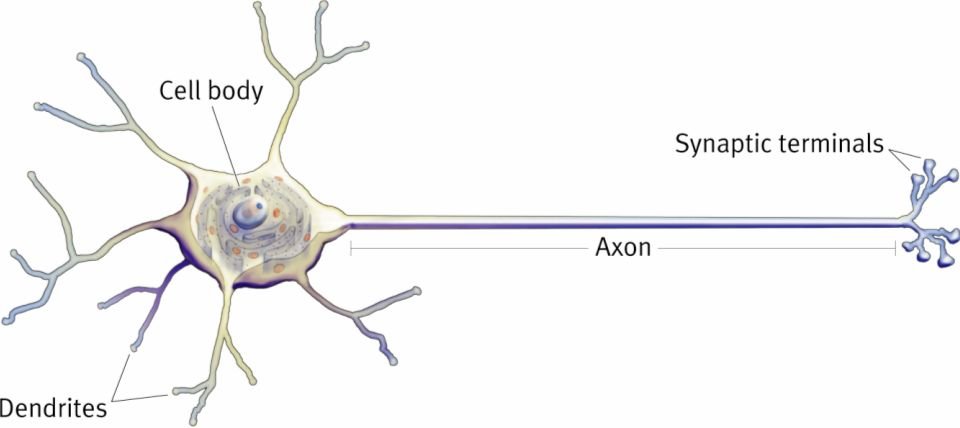
\includegraphics[width=0.8\textwidth,scale=1]{files/neuron.jpg}  
\caption{The parts of a nerve cell or neuron as shown in \cite{NEU}.}
\label{fig:neuron}
\end{figure}
\end{center}


\section{Mathematical formalisation}\label{sec:mcpitts}
During the second world war, research in computer technology has been promoted for the sake of military purposes. With the advent of computer technology, neural networks started to become significant as models of abstract automata. McCulloch and Pitt's 1943 published work (>>\textit{A logical calculus of the ideas immamnent in nervous activity}<<) proposes a cell which allows th simulation of AND-, OR- and NOT-gates and therefore every boolean function. This cell is a simple model of neuron with binary threshold and the first formal describtion of a neural network. Within their work, neurons are perceived as basic Input/Ouput units, which process input of $i$ neurons and propagate their output further into the network through a single output.\\

The activity level $a_j$ of a neuron $j$ is assigned by its transfer function $\varphi$. McCulloch and Pitt proposed a simple step function, where $S$ is the threshold:\\

\begin{equation}
	\varphi(x)=\begin{cases}
		0: \quad  x < S \\
		1: \quad  x \geq S \\
	\end{cases}
\label{eq:step}
\end{equation}
%The synaptic terminal's function is depicted by the multiplication of the input from neuron $a_i$ by a factor, the weight $w_{ij}$ of the connection link between neurons $i$ and $j$. $w_{ij}$ is either excitatory or inhibitory. 
Given the definition of $\varphi$ in equation \eqref{eq:step}, activity levels are always binary and computed as follows:\\

%\begin{equation}
%a_j = \varphi(\sum_{i=0}^{} w_{ij} \cdot a_{i}), \quad a_i \in \{0, 1\}, w_{ij} \in \{1, -1\}
%\end{equation}

\begin{equation}
a_j = \varphi(\sum_{i}^{} a_{i}), \quad a_i \in \{0, 1\}
\end{equation}

Figure \ref{fig:mathneuron} illustrates the mathematical formalisation proposed in \cite{NEURONMATH}. This model has later been named \textbf{McCulloch-Pitts neuron}. 


\begin{figure}
\centering

\begin{tikzpicture}
\node [align=center] (in1) at (-0.5,0) {$a_i$}; 
\node [align=center] (in2) at (-0.3,0.75)   {}; 
\node [align=center] (in3) at (-0.8,1.5) {$a_i = 1$}; 
%\node [align=center] (w1) at (0.7,0) {$w_{ij}$}; 
%\node [align=center] (w3) at (0.7,1.5) {$w_{0j}$};
\node [align=center] (input) at (2,0.75) {\ \ $\sum_{}^{in_{j}}$}; 
\node [align=center] (function) at (4,0.75) {$\varphi$}; 
\node [align=center] (output) at (6,0.75) {$a_j$}; 
%\node [align=center] (o1) at (8.5,0) {};
\node [align=center] (o2) at (8.5,0.75) {};
%\node [align=center] (o3) at (8.5,1.5) {};

\node [align=center] (desilinks) at (-0.60,-1) {Input\\ Links}; 
\node [align=center] (desinput) at (1.9,-1) {Input\\ funcion}; 
\node [align=center] (desfunc) at (4,-1) {Activation\\ function}; 
\node [align=center] (desoutput) at (6,-1) {Output}; 
\node [align=center] (desolinks) at (8,-1) {Output\\ link}; 

\node [align=center] (desweight) at (4,2) {$a_j = \varphi(in_j)$}; 
%\node [align=center] (desinfunc) at (0.75,2) {\small Weight}; 
\node [align=center] (descneuron) at (6,1.5) {\small Cell body}; 

\node [align=center] (dummy1) at (2.4,0.75) {}; 
\node [align=center] (dummy2) at (5.36,0.75) {}; 

\draw[arrow]	(in1) -- (input);
\draw[arrow]	(in2) -- (input);
\draw[arrow]	(in3) -- (input);

%\draw[arrow]	(output) -- (o1);
\draw[arrow]	(output) -- (o2);
%\draw[arrow]	(output) -- (o3);

\node[draw=black, fit=(dummy1) (function) (dummy2), ellipse] (tmp) {};

\end{tikzpicture}
\caption{A mathematical model of a neuron $j$}
\label{fig:mathneuron}
\end{figure}

This proposal is of particular importance for the theory of ANN and inspired significant researchers like John von Neumann or Nobert Wiener, who developed cybernetics. However, the McCulloch-Pitts neurons are limited by their inability to learn, resulting from their fixed structure. They also lack the surprising robustness of biological nerve networks, since they rely on a flawless operation of all components. Nevertheless, they still have significance in electrical engineering, where they are used to realise binary functions, due to their increased efficiency in contrast to gates. 

\chapter{Artificial neural networks}
\label{ch:ann}
\section{Overview}

Scientists have proposed a multitude of different network structures since the advent of research in ANN through their first formalisation. 
A lot of which have been designed with various motivations, stemming from the different perception of neural networks across disciplines.
Categorisation can be achieved by distinguishing several parameters, e.g. the number of layers, acceptance of input types or usage of learning techniques.
Figure \ref{fig:class} illustrates a possible categorisation\cite{NNGER}.
The direction of signal flow serves as a first level of distinction, as it substantially characterises the networks structure, complexity and so on.
Both types of signal flow mandate the propagation of network input further into the network.
Feed-forward network prohibit the usage of non-straightforward signal flow, i.e. connections may only emerge between subsequent neurons.
Any connections to predecessors are forbidden. This constraint has allowed for a quick development of learning techniques, empowering ANN to learn from data. 

As distinct from feed-forward networks, recurrent (or feedback) networks allow bidirectional signal flow. 
As links from one neuron may be formed with any other neuron in the network, recurrent network are often categorised by increased complexity.
Since the current state of a neuron may be continuously changing, recurrent networks demand advanced learning algorithms. \textbf{we?} We show an algorithm for training of recurrent network in section \ref{sec:btt}.
Due to their dynamic nature, they allow for the modelling of advanced techniques, such as long and short term memory.

\begin{figure}
\centering

\fbox{
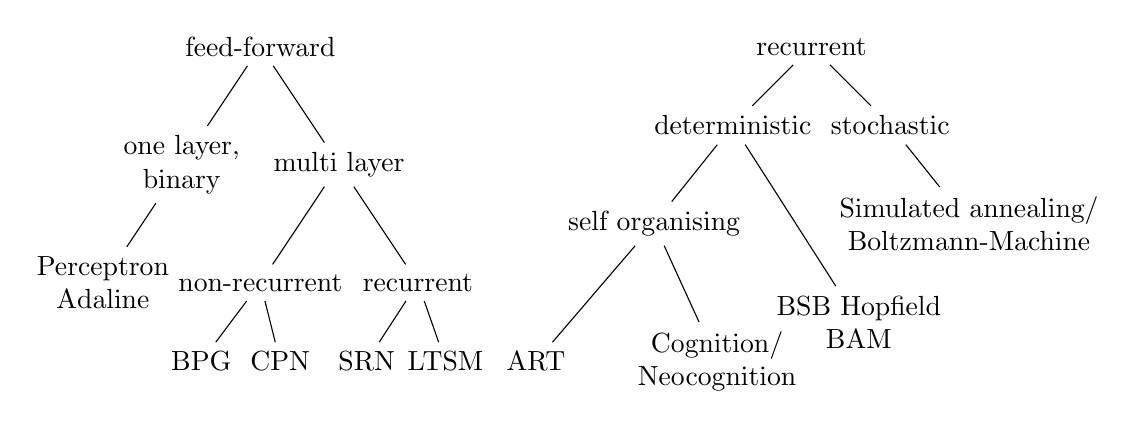
\begin{tikzpicture}
\node [align=center] (L1) at (3,10) {feed-forward}; 

\node [align=center] (R1) at (10,10) {recurrent}; 


\node [align=center] (L21) at (2,8.5) {one layer,\\ binary}; 
\node [align=center] (L22) at (4,8.5) {multi layer}; 

\node [align=center] (R21) at (9,9) {deterministic}; 
\node [align=center] (R22) at (11,9) {stochastic}; 


\node [align=center] (L31) at (1,7) {Perceptron\\Adaline}; 
\node [align=center] (L32) at (3,7) {non-recurrent}; 
\node [align=center] (L33) at (5,7) {recurrent}; 

\node [align=center] (R31) at (8,7.75) {self organising}; 
\node [align=center] (R32) at (10.6,6.5) {BSB Hopfield\\BAM}; 
\node [align=center] (R33) at (12,7.75) {Simulated annealing/\\Boltzmann-Machine}; 


\node [align=center] (L41) at (2.25,6) {BPG}; 
\node [align=center] (L42) at (3.25,6) {CPN}; \node [align=center] (L43) at (4.35,6) {SRN}; 
\node [align=center] (L44) at (5.35,6) {LTSM}; 

\node [align=center] (R41) at (6.5,6) {ART}; 
\node [align=center] (R42) at (8.80,6) {Cognition/\\Neocognition}; 

\foreach \s/\t in {L1/L21,
                   L1/L22,
                   L21/L31,
                   L22/L32,
                   L22/L33,
                   L32/L41,
                   L32/L42,
                   L33/L43,
                   L33/L44}
    \draw (\s) -- (\t);

\foreach \s/\t in {R1/R21,
                   R1/R22,
                   R21/R31,
                   R21/R32,
                   R22/R33,
                   R31/R41,
                   R31/R42}
    \draw (\s) -- (\t);

\end{tikzpicture}}
\caption{A categorisation of neural network types. BPG = Backpropagation, CPN = Counterpropagation, BAM = Bidirectional associative memory, BSB = Brain-State-in-a-Box, ART = Adaptive Resonance Theory, SRN = Simple recurrent network, LTSM = Long short term memory}

\label{fig:class}
\end{figure}
A comprehensive introduction of all categorised network types would exceed the scope of this project work, and therefore only a subset, interesting for the particular application, will be introduced. Within this chapter, we will give an introduction of the terminology and mathematical models used to represent a neural network on a computing machine. An appraisal of advantages and detriments of the presented models is rather difficult, as their performance hugly depends on the specific application. Regarding machine learning, and thereforea also ANN, the term performancedemands for a new definition. Machine learning is a scientific discipline that explores the construction and study of algorithms that can learn from data.\cite{MLDEF1} Such algorithms operate by building a model from example inputs and using that to make predictions or decisions.\cite{MLDEF2} As distict from other algorithms, there can never be absolute certainity of the correctness of a machine learning model. This stems from their usage of the probability of statistics applied to real world problems. Algorithmic measures, such as optimality and completeness cannot be utilised to assess the usefulness of a machine learning technique. A performance evaluation can therefore only be conducted given a specific problem and the according data. After all, the selection and appropriate usage of neural network structures requires extensive experience and/or thorough testing. 

\section{Network structure}
\subsection{Layers}
The units within a network are categorised into several layers according to their position. This allows for an accurate description of the network and the function of each respective unit within the network. The set of layers of a ANN will be denoted as $L$, where an artificial neural network of size n, written as $\text{ANN}^n$ is the union of the n layers in the network:

\begin{equation}
    \text{ANN}^n = \bigcup_{N}^{i=1}{L_i}
\end{equation}

The amount of neurons within a layer is equal to the elements of the respective set. The total number of neurons in an ANN is $\sum_{i=1}^{n}{|L_i|}$. The tuple $(|L_1|,...,|L_n|)$ is called the \textbf{network topolgy} and fully describes the structure (with exclusion of the connections) of a feed-forward network. Recurrent networks need and additional description.

The first network layer $L_1$, is referred to as the input layer. It receives the input vector $\overrightarrow{x} \in \mathds{R}^{|L_1|}$ and passes it onto the next layer. Likewise, $L_n$ is the output layer of the network, whose neurons are called the output units. $\overrightarrow{y} \in \mathds{R}^{|L_n|}$ is the output vector of an ANN. A computer application will later utilise the neural network as a black box, being only interested in the transformation from $\overrightarrow{x}$ to $\overrightarrow{y}$. Figure \ref{fig:layer} shows this. 

\begin{figure}
\centering

\begin{tikzpicture}
\node [draw=black, align=center, circle] (i1) at (0,3) {}; 
\node [draw=black, align=center, circle] (i2) at (0,2) {}; 
\node [draw=black, align=center, circle] (i3) at (0,1) {}; 
\node [draw=black, align=center, circle] (i4) at (0,0) {}; 

\node [draw=black, align=center, circle] (h01) at (2,2.5) {}; 
\node [draw=black, align=center, circle] (h02) at (2,1.5) {};
\node [draw=black, align=center, circle] (h03) at (2,0.5) {};

\node [draw=black, align=center, circle] (h1) at (4,2.5) {}; 
\node [draw=black, align=center, circle] (h2) at (4,1.5) {};
\node [draw=black, align=center, circle] (h3) at (4,0.5) {};

\node [draw=black, align=center, circle] (o1) at (6,2) {};
\node [draw=black, align=center, circle] (o2) at (6,1) {};

\draw[arrow]	(i1) -- (h01);
\draw[arrow]	(i1) -- (h02);
\draw[arrow]	(i1) -- (h03);

\draw[arrow]	(i2) -- (h01);
\draw[arrow]	(i2) -- (h02);
\draw[arrow]	(i2) -- (h03);

\draw[arrow]	(i3) -- (h01);
\draw[arrow]	(i3) -- (h02);
\draw[arrow]	(i3) -- (h03);

\draw[arrow]	(i4) -- (h01);
\draw[arrow]	(i4) -- (h02);
\draw[arrow]	(i4) -- (h03);

\draw[arrow]	(h1) -- (o1);
\draw[arrow]	(h1) -- (o2);

\draw[arrow]	(h2) -- (o1);
\draw[arrow]	(h2) -- (o2);

\draw[arrow]	(h3) -- (o1);
\draw[arrow]	(h3) -- (o2);

\node[draw=black,fit=(i1) (i2) (i3) (i4),ellipse] (inputLayer) {};
\node[draw=black,fit=(h01) (h02) (h03) ,ellipse] (hiddenLayer) {};
\node[draw=black,fit=(h1) (h2) (h3) ,ellipse] (hiddenLayer) {};
\node[draw=black,fit=(o1) (o2) ,ellipse] (outputLayer) {};

\node [align=center] (x) at (-1,1.5) {$\overrightarrow{x}$};

\node [align=center] (di) at (0,5) {\textcolor{black}Input\\ layer\\ $L_1$};
\node [align=center] (dh1) at (2,5) {\textcolor{black}Hidden\\ layer\\ $L_{2}$};
\node [align=center] (dh1) at (3,1.5) {$\cdots$};
\node [align=center] (dh2) at (4,5) {\textcolor{black}Hidden\\ layer\\ $L_{n-1}$};
\node [align=center] (do) at (6,5) {\textcolor{black}Output\\ layer\\ $L_n$};

\node [align=center] (y1) at (7,1.5) {$\overrightarrow{y}$};

\end{tikzpicture}
%\caption{%An example of an artificial neural network with $n$ layers. Its network topology is $(|L_1|=4,|L_2|=3,...,|L_{n-1}|=3,|L_n|=2)$}
\label{fig:layer}
\end{figure}

Particular significance is drawn to the layers in between input and output layer. Those layers are optional, but needed to solve certain problems. We will discuss the importance of hidden layers for problem solution in chapter \ref{chap:nets}. We denote the set of hidden layers as $H$. It is described as follows:
\begin{equation}
H \subseteq L; H = \{L_i|1<i<n\}
\end{equation}

\subsection{Units}
\label{subsec:weights}

A first improvement to McCulloch and Pitt's model was the concept of weights on the connecting links. Inspired by the function of the synaptic 
terminals, a weight $w_{ij}$ between two neurons $n_i$ and $n_j$, models the magnitude of influence. Weights may be both positive and negative, 
exhibatory or inhibatory. A magnitude of zero stands for a cut-off signal flow. The entirety of connection weights within a network is often stored 
in a matrix, which allows for cheap manipulation of the weights. 
The manipulation of connections weight may be used to alter the network's behaviour. $W$ is called the connection matrix, which fully represents 
the structure of a feed-forward network with $i$ layers:
\begin{equation}
W = 
\begin{pmatrix}
w_{11} & \cdots & w_{i1} \\
\vdots & \ddots & \vdots \\
w_{1j} & \cdots & w_{ij} \\
\end{pmatrix}
\end{equation}

In addition, the concept of bias neurons has proven itself useful. Bias units are non-receptive, both in feed-forward and recurrent networks. Hence their activity level is steady, usually $+1$. Links between bias and normal neurons are to be treated normally, the influence of a bias can therefore be altered. They are often used to keep units with little weighted input active, by shifting their activation function $\varphi$ they don't receive significant input. In contrast, a negative link may be used to keep a neuron in an inactive state.
\begin{figure}
\centering

\begin{tikzpicture}
    \node [draw=black, align=center, circle] (i) at (0,0) {$n_0$}; 
    \node [draw=black, align=center, circle] (o) at (4,0) {$n_1$}; 

    \draw[arrow]	(i) -- (o);

    \node[] (dw) at (2,0.3){$w_{ij}$};
    \node[] (di) at (0,0.6){Input: $x$};
    \node[] (do) at (4,0.6){Output};
    \node[] (df) at (2.1,-0.7){$\varphi = sig(w_{01}\cdot x)$};
\end{tikzpicture}

\caption{A single input-output network}
\label{fig:1on1}
\end{figure}

Consider the network shown in figure \ref{fig:1on1}. The activation function of the output neuron is chosen to be the sigmoid function. Figure \ref{fig:sigmoid-scale} shows the output for several values of $w$. It can seen that $w$ changes the steepness of the sigmoid function. 

\begin{figure}
    \centering
    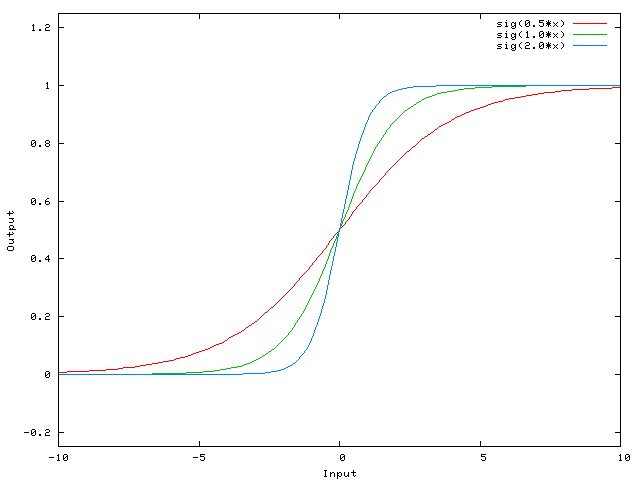
\includegraphics[width=0.65\textwidth,scale=1]{files/sigmoid-scale.png}  
    \caption{The output of unit $n_1$ in figure \ref{fig:1on1}}
    \label{fig:sigmoid-scale}
\end{figure}


Figure \ref{fig:2on1} shows the same network with an additional bias neuron. This allows us to shift the activation function according to the weight of the connection link $w_{12}$ as shown in figure \ref{fig:sigmoid-shift}.

\begin{figure}
\centering
    \begin{tikzpicture}
    \node [draw=black, align=center, circle] (i2) at (0,2) {$n_0$}; 
    \node [draw=black, align=center, circle] (i1) at (0,0) {$n_1$}; 
    \node [draw=black, align=center, circle] (o) at (4,1)  {$n_2$}; 

    \draw[arrow]	(i2) -- (o);
    \draw[arrow]	(i1) -- (o);

    \node[] (dw) at (2,1.8){$w_{02}$};
    \node[] (dw) at (2,0.8){$w_{12}$};
    \node[] (di) at (0,0.6){Bias: $1.0$};
    \node[] (di) at (0,2.6){Input: $x$};
    \node[] (do) at (4,1.6){Output};
    \node[] (df) at (2.1,-0.7){$\varphi = sig(w_{02}\cdot x + w_{12}\cdot 1.0)$};
    \end{tikzpicture}
\caption{A single input-output network}
\label{fig:2on1}
\end{figure}

\begin{figure}
    \centering
    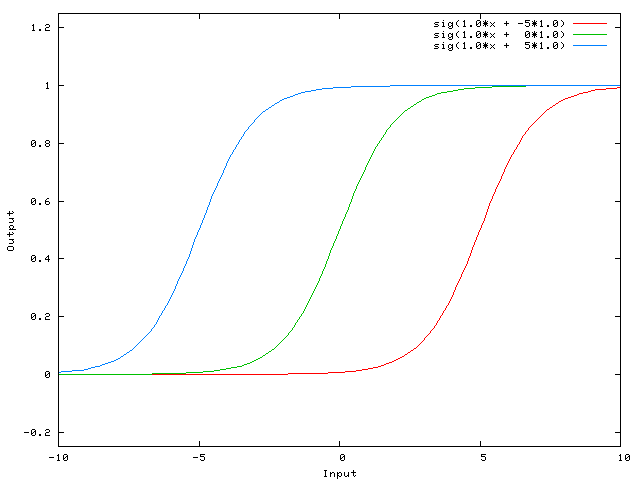
\includegraphics[width=0.65\textwidth,scale=1]{files/sigmoid-shift.png}  
    \caption{The output of unit $n_1$ in figure \ref{fig:2on1}}
    \label{fig:sigmoid-shift}
\end{figure}

\subsection{Activation functions}

As discussed before, the weights of the connections between the neurons represent the 'Intelligence' of the network. The bigger the absolute value of the weight, the greater the influence of a neuron to another. This value can be both positive and negative, as well as neutral \textit{(0)}, meaning that there is currently no influence between the neurons, although there is still a link connecting them. A weight of 0 can be understood as a logical pinch of the link, preventing it from transmitting signals.


The connection between the input values and the activity level of the neuron is made by the activity function $\varphi$. Different models are obtained depending on the choice of the activity or transfer function. Amongst the most common choices are the linear, binary step and sigmoid function as illustrated in Figure \ref{fig:plots}. The linear function has a threshold $t$, which can be used to avoid low network input (e.g. noise) to be further propagated into the network. The binary step function represents the firing of a pulse down the axon if positive $1$), while $0$ represents no firing. The step function is sometimes defined to jump from $-1$ to $1$. 

Sigmoid functions are widely used amongst network which are to represent cognitive processes such as perception, recognition, problem solving, etc. .
Both the logistic function as well as the hyperbolic tangent function $\tanh()$ can be used. The main advantage of sigmoid functions are:

\begin{itemize}
\item In contrast with the linear function (without a threshold), the activity level of the function is limited in both the positive and the negative. This means that activity in the network can not spill over unintentionally, which can be caused by recurrent connections.
\item Differentiability
As distinct from the binary step function, it is differentiable at all parts, which as an example, is a requirement of the gradient descent, used by the Backpropagation algorithm (about to be introduced in chapter \ref{ch:learning}
\end{itemize}


\begin{figure}
\centering
\subfigure[]
{
   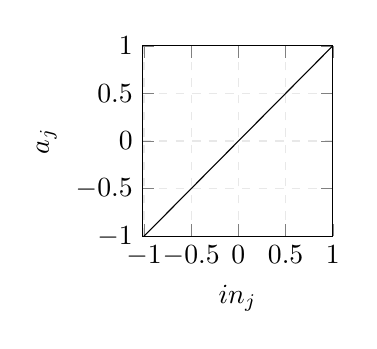
\begin{tikzpicture}
		\begin{axis}[
        width=4cm, height=4cm,
        grid = major,
        grid style={dashed, grey!30},
		xmax=1,        
        ymin=-1,
        ymax=1,
        axis background/.style={fill=white},
        ylabel=$a_{j}$,
        xlabel=$in_{j}$]
     
		\addplot[black]{x};
		\end{axis}
	\end{tikzpicture}
\label{fig:plot1}
}

\subfigure[]
{
   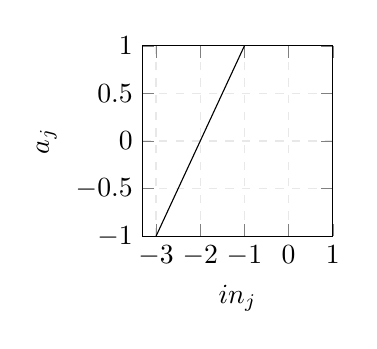
\begin{tikzpicture}
		\begin{axis}[
        width=4cm, height=4cm,
        grid = major,
        grid style={dashed, grey!30},
		xmax=1,        
        ymin=-1,
        ymax=1,
        axis background/.style={fill=white},
        ylabel=$a_{j}$,
        xlabel=$in_{j}$]
     
		\addplot[black]{x+2};
		\end{axis}
	\end{tikzpicture}
\label{fig:plot2}
}

\subfigure[]
{
   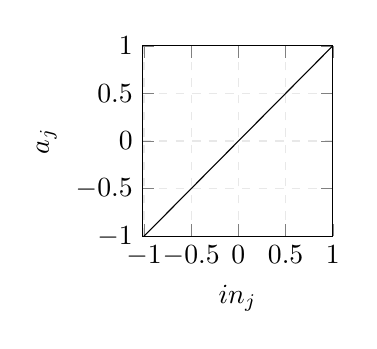
\begin{tikzpicture}
		\begin{axis}[
        width=4cm, height=4cm,
        grid = major,
        grid style={dashed, grey!30},
		xmax=1,        
        ymin=-1,
        ymax=1,
        axis background/.style={fill=white},
        ylabel=$a_{j}$,
        xlabel=$in_{j}$]
     
		\addplot[black]{x};
		\end{axis}
	\end{tikzpicture}
\label{fig:plot2}
}
	
\caption{Comparison of commonly used activation functions}
\label{fig:plots}
\end{figure}

In order to teach neural networks and enable them to apply learned behavior in following scenarios, the work with them is divided in a training- and test phase. During the training, the network learns certain behavior by feeding repetitive input to the first layer and observing the output of the network. This can be done in a supervised and unsupervised way. In a supervised training phase, the targeted output of the network is already known and is presented to the network as a \textit{teaching factor}. The network produces output depending on the current weights on its connections and adjusts them according to the margin between the targeted and produced output. Unsupervised learning is necessary in situations, where no reasonable teaching factors are available or the observant is more interested on the performance. Similarity between input incentives and connection weights is the factor, according to which weight adjustment is done in such models.

\section{Applications}
\label{sec:exp}
Until today, neural networks have been successfully applied to several problems in a variety of scientific and industrial applications. Although of greatly different nature, almost all of those applications can be reduced to either pattern/shape recognition or logical filter tasks. Examples are:\\
\begin{itemize}
    \item On-line recognition of handwritten text
    \item Autopilots in aerospace engineering
    \item Noise suppression and signal filtering in communication technology 
    \item Object recognition
    \item Weather forecast
    \item Function approximation including time series prediction
\end{itemize}

The following sections will give a brief notion of some 'classical' applications where ANNs have found better solutions in shorter time in comparison with other techniques.
\subsection{Recognition of hand-writing}
The automated interpretation of hand-written is of great interest for a number of purposes. The destination address of letters and parcels are nowadays processed by computers which use real-time image processing system to recognize handwriting on letters. The typesetting system \LaTeX  allows its users to phrase complex formulas using certain commands which are later being replaced by symbols such as the existential quantifier $\exists$. 
One would now wish for a system that can take in a hand written representation of the symbol and output the command by which the symbol can later be written in a document. In \cite{MARTIN} artificial neural networks are used to classify such symbols. After drawing the sought symbol, the user is presented a choice of matching symbols along with an associated probability measure of their correctness. The website is available under \url{write-math.com}.
\\

The challenge for such systems is the great deviation of styles in hand-written text. This makes it virtually infeasible for conventional methods to reliably classify hand-writing. 
The network model RCE(Restricted Coulomb Energy Network) has been devised by Nobel price winner Leon Cooper. It overcomes the limitations of the Perceptron as it is capable of detecting geometrical figures (therefore also handwritten text) of any size. 
Cooper's company Nestor, has successfully used this model to develop a system which can detect characters of the Japanese alphabet Kanji. The Kanji alphabet stems from the Chinese language, contains approximately 3000 different symbols and is extremely complex. 
Examples are \begin{CJK}{UTF8}{min}輸\end{CJK} - transport or \begin{CJK}{UTF8}{min}熊\end{CJK} - bear. It is nowadays extensively used on mobile devises that allow to write text messages by drawing each individual character instead of choosing symbols from a massive dictionary. 
Complex sentences formulated by simultaneously using three different alphabets, such as \begin{CJK}{UTF8}{min}世界はコンピュータ技術の登場以来、劇的に変化した。\end{CJK} - \textit{The world has changed dramatically since the advent of computer technology} can now be written in a fairly short amount of time.

\subsection{The Travelling-Salesman-Problem}
Given a set of cities and the distances between each pair of cities, what is the shortest path that, after visiting each city exactly once, leads to the origin of the route? This task, called the Travelling-Salesman-Problem (often abbreviated as TSP) is an optimisation task which is often encountered in practice (Energy and water supply, microchip design). The TSP can be modelled as a graph: All $n$ cities are represented as vertices, the connections between the cities as edges. Since all cities are connected with each other, the graph is complete. A complete graph is called $K_n$. The cost (travel time) between each pair of vertices $i$ and $j$ is associated with a weight $w(i,j) \geq 0$. A tour that visits each city once and return back to the origin is a Hamilton-circle. As the graph is complete, there are several Hamilton-circles (each of which is a possible solution of the problem). Each permutation of the nodes is a Hamilton-circle, thus there are $n!$ circles. Sought is the Hamilton-circle with the least overall cost, i.e. a permutation $\pi(1),\dots,\pi(n)$ with minimal weight
\begin{equation}
    \sum\limits_{i=1}^n w(\pi(i),\pi(i+1)), 
\end{equation}

where $\pi(n+1)$ is set to $\pi(1)$.\cite{MATHINF}\\

It is of high importance to theoretical computer science, as it is known to be $NP$-complete. In the field of complexity analysis, the class of decision problems for which there is a deterministic Turing-Machine able to solve it in time $\mathcal{O}(n^k)$ is called $P$ (polynomial). An example is the sorting problem. Class $P$ contains problems with running times like $\mathcal{O}(n)$ and $\mathcal{O}(log(n))$ but also those with time $\mathcal{O}(n^{5000})$. In addition to the deterministic Turing machine, complexity analysis also defines the non-deterministic Turing machine. At each time step, there are several possible ways of continuing computation, setting it in contrast with todays computers. The class of Problems $NP$ is solvable by a non-deterministic Turing Machine in polynomial time. $NP$ contains a number of relevant problems, such as the graph isomorphism (Can two graphs be drawn identically?). Problems in $P$ can also be solved by this theoretical model, so $P \subseteq NP$. In other words, a problem is in the class of NP if there is an algorithm (executed by a Turing machine) that can guess a solution and verify whether the guess was correct in polynomial time. In case of omniscient guessing or given a number of processors equal to the number of solutions, trying out all possibilities at the same time one would always get the correct solution. Thus, $NP$ problems would become $P$ problems. 

Nevertheless, computationally feasible approximation techniques have been found which allow to find a good, although not always the best, solution. Hopfield and Tank (1985) proposed an approach using ANNs which allows to find a good, often even the best solution for the TSP. It suggests a single-layer network with $n$ neurons, where $n$ equals the number of cities in the graph, called Hopfield-network. This can be thought of as a square with an edge length of $n$. The output of each individual neuron equals the time step at which the city is visited. Furthermore, genetic algorithms have also been applied to find an approximate solution for the problem %\cite{GENTSP}.


\chapter{Learning}\label{ch:learning}
\section{Hebbian learning rule}
The psychologist Donald Olding Hebb proposed on the easiest learning rules with high biological plausibility in \cite{HEBB}:\\

\textit{“Let us assume that the persistence or repetition of a reverberatory activity (or "trace") tends to induce lasting cellular changes that add to its stability.… When an axon of cell A is near enough to excite a cell B and repeatedly or persistently takes part in firing it, some growth process or metabolic change takes place in one or both cells such that A's efficiency, as one of the cells firing B, is increased.”}\\

In summary: The weight between two units $i$ and $j$ is changed, if both units are active at the same time. The amount of change is set by three factors:

\begin{itemize}
\item The activity level of the sending unit $a_i$.
\item The activity level of the receiving unit $a_j$.
\item A settled and constant parameter $\eta$
\end{itemize}

The weight change $\Delta w_{ij}$ using the bias learning rule is shown in equation \eqref{eq:hebb}.
\begin{equation}
\Delta w_{ij} = \eta \cdot a_i \cdot a_j
\label{eq:hebb}
\end{equation}

One of the major drawbacks of the Hebbian rule is the fact, that is can only applied on networks without a hidden ayer, and therefore only very simple neural networks.

\section{Delta rule}
The delta rule is based on the comparison between a targeted output $t$ and the observed output $o$ and can therefore only be applied with supervised learning.
It can be expressed using equation \eqref{eq:delta1}.
\begin{equation}
\delta = t - o
\label{eq:delta1}
\end{equation}

The following possibilities can be observed:
\begin{itemize}
\item \textbf{The observed output is too low}\\
In order to amplify the output, the weights between neurons is strengthened, provided a positive weight on the connection linking them. Negative weights are weakened.
\item \textbf{The observed output is too high}\\
All connections with positive weights are weakened, while the ones with negative weights are strengthened 
\item \textbf{Targeted and observed output are equivalent. (= ideal behavior)}\\ There is no need to change the links.
\end{itemize}

The deltas learning rule equation \eqref{eq:delta2} covers all three possibilities, thus ensuring that the changing rate is proportional to the difference between targeted and observed. The learning parameter $\eta$ is again set before the beginning of the learning process and remains constant. The multiplication with the sending units output $a_i$ ensures that those connections, that have the greatest influence into the error have the greatest $\delta w_{ij}$.
\begin{equation}
\Delta w_{ij} = \eta \cdot \delta \cdot a_i
\label{eq:delta2}
\end{equation}

The simplicity of this learning rules also comes at great cost: The comparison only allows us to adjust connections which connect to the rightmost layer in the network. This fact restricts the application of this method from networks with a hidden layer. 

\section{Backpropagation}

\subsection{Gradient descent}

The optimisation algorithm gradient descent (also steepest descent) tackles the problem of finding a local minimum of a multivariable function $F(x)$. In order to do, one substracts the gradient $\nabla F(a)$ from the current point $a$ to obtain a new point $b$ so that $F(a) \geq F(b)$. The non-negative weight $\gamma$ is often referred to as the stepsize.

\begin{equation}
 b = a - \gamma \nabla F(a)
\label{eq:graddes}
\end{equation} 

The gradient of a differentiable function $f: D \subseteq \mathds{R}^n$ $\rightarrow$ $\mathds{R}$ must disappear at a local minimum or maximum at $x_i$:\cite{MATHINF}

\begin{equation}
\nabla F(x_i) = 0
\end{equation} 

Starting with guess $x_0$ for a local minimum, and iteratively calculating an $x_{i+1}$ according to equation \eqref{eq:graddes}, we will obtain $x_0, ..., x_i$ so that $F(x_0) \geq F(x_1) \geq ... \geq F(x_{n-1}) \geq F(x_n)$. The parameters $\theta$ and $n$ are  used as an ending criteria for the algorithm. Algorithm \ref{alg:GD} shows the complete algorithm.

\begin{algorithm}
\LinesNumbered
\DontPrintSemicolon
\BlankLine
\Ein{A differentiable function $F(x)$, step size $\gamma$, tolerance $\theta$, point $x_0$}
\Aus{A local minimum at $x_i$}
\BlankLine
\Begin
{
    \Repeat{$\Delta x < \theta$ for $n$ iterations}
    {
        $x_{i+1}$ = $x_i - \gamma \nabla F(x_i)$
    }
}
\caption{The gradient descent algorithm}
\label{alg:GD}
\end{algorithm}

Gradient descent may be imagined as the effort of a wanderer to reach the bottom of valley as quick as possible, therefore always seeking to climb down as the point of steepest descent. This is illustrated in Figure \ref{fig:grad}

\begin{figure}
    \centering
    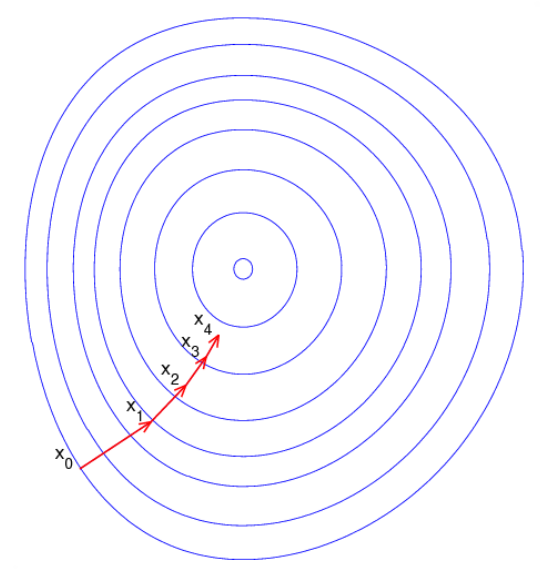
\includegraphics[width=0.3\textwidth,scale=1]{files/graddes.png}  
    \caption{Illustration of gradient descent.\cite{GRADFIG}}
    \label{fig:grad}
\end{figure}

\subsection{The Backpropagation algorithm}

The Backpropagation algorithm is yet another learning rule for supervised networks, but in comparison to the Hebbian and delta rules, it can also be applied for networks with $n$ numbers of hidden layers. There are certain problems that cannot be solved by networks without at least one hidden layer, the XOR-Gate being a famous example. 
It was developed by several scientists simultaneously \cite{BACK1}\cite{BACK2}\cite{BACK3} and consists of three stages:
\begin{itemize}
\item[1.] \textbf{The forward-pass}:
A pattern is presented to the input layer and further propagated into the network.
\item[2.] \textbf{Error-determination}:\\
The observed output is compared to targeted result and an error $E$ is determined by a derivable error-function $\varphi$ shown in equation \eqref{eq:backerror}. The factor of $\frac{1}{2}$ is used to simplify the derivation by cancelling the exponent.

\begin{equation}
\varphi = \frac{1}{2} (t-o)^2
\label{eq:backerror}
\end{equation}
\item[3.] \textbf{Backward-pass}:\\
The error is propagated from the back of the network to the front, hence the name \textbf{Backpropagation}. The connection are updated independent from their influence to $E$, which guarantees a result $o$ that is closer to $t$, provided the same output is presented to the input layer.
\end{itemize}

A first approach on finding a method to changing all weights in a weight that will minimize the error is to find $E$ for all possible combinations of weights $W$. The combination $W_{min}$ with the smallest $E$ would be the perfect solution, an absolute minimum of the error. The problem of this approach is that the computational effort to finding this solution is way to high, since $W_{min}$ would have to be found in a $n$-dimensonial  hyperplane (given the number of neurons $n$).\\

Instead, the weights are adjusted using the gradient descent, which does not need to know the complete hyperplane\marginpar{\textit{gradient descent}}. It starts with a random combination of weights for which the gradient is determined. The gradient is the function of a scalar field which shows the rate of change and the direction of the greatest change in the form of a vector field. After the gradient is determined it will be stepped down at a given rate - the learning rate, meaning that the weights are adjusted. For this new combination of weights, the gradient is again determined and stepped down until a local (or global minimum) is found or a maximum amount of repetitions is reached.\\

The amount of change between neurons $i$ and $j$ $\delta w_{ij}$ is calculated as shown in \eqref{eq:backrule}.
\begin{equation}
\Delta w_{ij} = -\eta \frac{\partial E}{\partial w_{ij}} = \eta \cdot \delta_j \cdot a_i
\label{eq:backrule}
\end{equation}
As distinct form the delta rule, the Backpropagation rule differs two cases, shown in equation \eqref{eq:backcases}. $k$ is the index of the neurons in the subsequent layer.
\begin{equation}
   \delta_j =
   \begin{cases}
     \varphi'(in_j)(t_j-o_j) & \text{In case j is an output neuron} \\
     \varphi'(in_j)\sum_{k} \delta_k \cdot w_{j,k} & \text{In case j is a hidden neuron}
   \end{cases}
\label{eq:backcases}
\end{equation}

Eventually, the weights are changed according to equation \eqref{eq:backweight}.

\begin{equation}
   w_{ij}^{new} = w_{ij}^{old} + \Delta w_{ij}
\label{eq:backweight}
\end{equation}

% \section{Backpropagation through time}
% 
% The Backpropagation through time (BTT) algorithm constitutes a learning rule for recurrent networks. 
% Recurrent networks constitute an architecture that allows bi-directional signal flow within the network. While outputs of feed-forward networks are restricted to be only connected to 
% a neuron in the preceding layer, connections can now be formed across arbitrary layers. Figure \ref{fig:feedback} shows a recurrent network. As the neuron is connected with
% itself, it forms a feedback structure. The output of the neuron at time step $t$ serves as a weighted (by weight $g$) input of itself in the next time step.
% Thus, the output of the network can be computed as follows:
% 
% \begin{equation}
%     y(t+1) = \varphi(w\cdot x(t) + g\cdot y(t))
% \label{eq:btt}
% \end{equation}
% 
% BTT was independently developed by several researchers.%\cite{BTT1}\cite{BTT2}\cite{BTT3}
% Back
% 
% 
% \begin{figure}
% \centering
%     \begin{tikzpicture}
%     \node [align=center] (l1) at (0,0) {}; 
%     \node [align=center] (x2) at (0.0,0.3) {$x(t)$}; 
%     \node [align=center] (x1) at (0.75,0.3) {$w$}; 
%     \node [draw=black, align=center, circle] (n) at (1.5,0) {}; 
%     \node [align=center] (x2) at (2.95,0.3) {$y(t+1)$}; 
%     \node [align=center] (x3) at (1.6,-0.7) {$g$}; 
%     \node [align=center] (l2) at (3,0) {}; 
% 
%     \draw[arrow]	(l1) -- (n);
%     \draw[arrow]	(n) -- (l2);
%     \draw[arrow] (n) to [out=330,in=250,looseness=8] (n);
%     \end{tikzpicture}
% \caption{A feedback structure in a recurrent neural network.}
% \label{fig:feedback}
% \end{figure}
% 
% \begin{figure}
% \centering
%     \begin{tikzpicture}
%     \node [align=center] (n0) at (0,0) {}; 
%     \node [] (y0) at (0.75,0.3) {$y(0)$}; 
% 
%     \node [] (g1) at (0.75,-0.2) {$g$}; 
%     \node [] (w1) at (1.50,0.7) {$w$}; 
%     \node [] (x1) at (1.0,1.3) {$x(0)$}; 
%     \node [] (t1) at (1.5,-0.7) {$t-1$}; 
%     \node [] (y1) at (2.25,0.3) {$y(1)$}; 
%     \node [draw=black, align=center, circle] (n1) at (1.5,0) {}; 
% 
%     \node [] (g2) at (2.25,-0.2) {$g$}; 
%     \node [] (w2) at (3.00,0.7) {$w$}; 
%     \node [] (x2) at (2.5,1.3) {$x(1)$}; 
%     \node [] (t2) at (3,-0.7) {$t-2$}; 
%     \node [] (y2) at (3.75,0.3) {$y(2)$}; 
%     \node [draw=black, align=center, circle] (n2) at (3,0) {}; 
% 
%     \node [] (g3) at (3.75,-0.2) {$g$}; 
%     \node [] (w3) at (4.50,0.7) {$w$}; 
%     \node [] (x3) at (4.0,1.3) {$x(2)$}; 
%     \node [] (t3) at (4.5,-0.7) {$t-3$}; 
%     \node [] (y3) at (5.25,0.3) {$y(3)$}; 
%     \node [draw=black, align=center, circle] (n3) at (4.5,0) {}; 
% 
%     \node [] (g4) at (5.25,-0.2) {$g$}; 
%     \node [] (w4) at (6.00,0.7) {$w$}; 
%     \node [] (x4) at (5.5,1.3) {$x(3)$}; 
%     \node [] (t4) at (6.0,-0.7) {$t-4$}; 
%     \node [] (y4) at (6.75,0.3) {$y(4)$}; 
%     \node [draw=black, align=center, circle] (n4) at (6,0) {}; 
% 
%     \node [] (g5) at (6.75,-0.2) {$g$}; 
%     \node [] (w5) at (7.50,0.7) {$w$}; 
%     \node [] (x5) at (7.0,1.3) {$x(4)$}; 
%     \node [] (t5) at (7.5,-0.7) {$t-5$}; 
%     \node [] (y5) at (8.25,0.3) {$y(5)$}; 
%     \node [draw=black, align=center, circle] (n5) at (7.5,0) {}; 
% 
%     \node [align=center] (n6) at (9,0) {}; 
% 
%     \draw[arrow]	(n0) -- (n1);
%     \draw[arrow]	(x1) -- (n1);
%     \draw[arrow]	(n1) -- (n2);
%     \draw[arrow]	(x2) -- (n2);
%     \draw[arrow]	(n2) -- (n3);
%     \draw[arrow]	(x3) -- (n3);
%     \draw[arrow]	(n3) -- (n4);
%     \draw[arrow]	(x4) -- (n4);
%     \draw[arrow]	(n4) -- (n5);
%     \draw[arrow]	(x5) -- (n5);
%     \draw[arrow]	(n5) -- (n6);
%     \end{tikzpicture}
%     \caption{The recurrent network shown in figure \ref{fig:feedback} during unfolding with depth $t=5$.}
% \label{fig:unrolled}
% \end{figure}
% 
% \begin{algorithm}
% \LinesNumbered
% \DontPrintSemicolon
% \BlankLine
% \Ein{Input $x(t)$ at time $t$, depth $k$}
% \Aus{Output $y(t)$}
% \BlankLine
% \Begin
% {
%     Unfold network to contain $k$ instances.\\
%     $y(0) \leftarrow \text{zero-magnitude vector} \overrightarrow{0}$.
%     
%     \For{$\forall t \in [0,n-1]: t \in \mathbb{N}_0$}
%     {
%         \tcp{Done for each }
%         Set network inputs $y(0), x(1), x(2), x(3)$\\
%         Forward-propagate.\\ 
%         Error $e = y(t+k) - t;$ $t:$ target error\\
%         Backpropagate the error across the whole unfolded network.\\
%         Update all the weights in the network according to standard Backpropagation.\\
%         $y(0) \leftarrow f(x)$
% 
%     
%     }
% }
% \caption{The Backpropagation through time algorithm.}
% \label{alg:GD}
% \end{algorithm}
% 
\section{Genetic algorithms}
\textit{Since this project builds off of Schembri's work, we assume knowledge about the hill-climbing approach in unsupervised learning used in \cite{DANIEL}. Readers not
familiar with hill-climbing and artificial evolution are advised to refer to the original paper before further reading.} 

\subsection{Crossover}
The unsupervised training of neural networks is greatly inspired by evolution. The notion of natural selection was first presented by Charles Darwin in his book “\textit{On the origin of species by means of natural selection}”\cite{DARWIN}. 
As a comprehensive discussion of Darwin's ideas lies out of the range of this paper, \textbf{we?} we will from here on refer to evolution as the following definitions\cite{OXFORD}:

\begin{center}
\textit{“Change in the genetic composition of a population during successive generations, often resulting in the development of new species. The mechanisms of evolution include natural selection acting on the genetic variation among individuals, mutation, migration, and genetic drift.”}\\
\end{center}

and

\begin{center}
\textit{“A gradual process in which something changes into a different and usually more complex or better form.”}\\ 
\end{center}

In particular, we are especially interested in a change or modification which results in a new entity (neural network) better accustomed to the 
respective demands of the environment.  We rate an ANN as better accustomed when its performance measure (i.e. the fitness function) has become 
higher. The hill-climbing algorithms tries to achieve this by modifications which continuously alter the weights of the respective network so 
as to maximise performance. However, this method may not reach a global maximum in case of local minima or flat parts of the respective fitness 
function.

Crossover spins the idea of artificial evolution further, still. Instead of merely keeping the best individual of each population and modifying 
its weights slightly in hope for better results, crossover implements the idea of artificial reproduction. Reproduction is implemented by a 
combination of the weights of two chosen networks according to specific criteria. The Crossover algorithm is usually used alongside hill-climbing 
to overcome the pitfall of local minima. We will refer to this combination of as \textit{augmented genetic algorithm}.

Figure \ref{fig:ag} shows the principle structure of the augmented genetic algorithm. A thorough explanation is also given in \cite{CROSSOVER}.
After a population has been applied in an environment, the fitness of each individual is ranked according to their performance.  
In addition, a selection process choses certain networks according to a selection function. Individuals are either selected for reproduction 
or direct mutation. Direct mutation is often used to clone the best-performing networks of the current population (sometimes called elitism). 
In case of direct mutation, the augmented genetic algorithm does not differ from the standard hill-climbing approach.

\paragraph{Selection}
%TODO: AI basics book cittation, figure
In selection, one might be inclined to presume that only well-performing agents ought to be taken into consideration for mating. However, creating
offspring from both a well and a poorly performing agents can help to increase the perormance. This is why none
of the networks must be excluded from the selection process. However, a bias towards better fitness is still desirable. This is implemented by 
increasing the chance of picking a better agents at random. One might think of the selection process of a game of roulette, where the sizes of the
fields vary. Each field stands for a network of the previous population, their size corresponds to their fitness. As in standard-roulette, each
field may be chosen, some with a higher probability than others. The roulette wheel is showin in \ref{fig:roul}.

\paragraph{Reproduction}
If two individuals are chosen for reproduction, they create a certain amount of children according to the rule of genetic combination. 
As an analogy to human reproduction, the selected networks will be referred to as the male and female part. Figure \ref{fig:repro} illustrates 
this process. One-Point Crossover is an example of a combination rule for two children.
During the mating process, a random integer, called crossover point ($CP$), is chosen. It determines the ratio of male and female genes in the offspring. 
Given that number, the genetic combination can finally take place.  When we talk about genes in the context of ANN, we usually mean the weights 
of the respective network. The crossover point simply states the number connection weights which are cloned from each parent to form the offspring.
The total number of weights in an ANN is equal to the number of elements in the weight matrix $W$ (see \ref{subsec:weights}) and can be calculated 
as follows: $|W| = \sum^{n-1}_{i=1} L_i \cdot L_{i+1}$.
$CP$ is then equal to the number of weights taken from the first parent, while $|W|-CP$ states the amount from the second parent. 

Other crossover rules are two point crossover, uniform crossover where genes are copied at random 
%\cite{UNIFORMCROSSOVER} and selective crossover\cite{SELECTCROSSOVER}.

\begin{figure}
	\centering
	\begin{tikzpicture}
	\node [draw=black, fill=white, align=center] (g) at (2,0) {Generation of initial individuals};
	\node [draw=black, fill=white, align=center] (e) at (2,-1) {Application};
	\node [draw=black, fill=white, align=center] (r) at (2,-2) {Fitness ranking};
	\node [draw=black, fill=white, align=center] (s) at (2,-3) {Selection};
	\node [draw=black, fill=white, align=center] (c) at (0,-4) {Crossover};
	\node [draw=black, fill=white, align=center] (m) at (4,-4) {Mutation};

	\draw[arrow]	(g) -- (e);
	\draw[arrow]	(e) -- (r);
	\draw[arrow]	(r) -- (s);
	\draw[arrow]	(s) -- (c);
	\draw[arrow]	(s) -- (m);
	\draw[arrow]	(c) -- (m);
    \draw[arrow]    (c) to[out=-180,in=-180] (e);
    \draw[arrow]    (m) to[out=0,in=0] (e);
	
	\end{tikzpicture}
    \caption{The principle structure of the augmented genetic algorithm.\cite{CROSSOVER}}
	\label{fig:ag}
\end{figure}

\begin{figure}
	\centering
	\begin{tikzpicture}
	\node [] (label) at (-2,0) {Parents};
	\node [draw=black, fill=white, align=center, circle] (m) at (0,0) {\mars};
	\node [draw=black, fill=white, align=center, circle] (f) at (3,0) {\female};

    \node [draw=black, fill=white, align=center] (co) at (1.5,-1) {Crossover};

	\node [] (label) at (-2,-2) {Children};
	\node [draw=black, fill=white, align=center, circle] (c1) at (0,-2) {1};
	\node [draw=white, fill=white, align=center] (c2) at (1.5,-2) {\dots};
	\node [draw=black, fill=white, align=center, circle] (c3) at (3,-2) {n};

	\draw[arrow]	(m) -- (co);
	\draw[arrow]	(f) -- (co);
	\draw[arrow]	(co) -- (c1);
	\draw[arrow]	(co) -- (c2);
	\draw[arrow]	(co) -- (c3);
	
	\end{tikzpicture}
	\caption{An illustration of the crossover reproduction model. Two parent networks are unified two create offspring.}
	\label{fig:repro}
\end{figure}

\begin{figure}
    \begin{center}
        $
        W_{\mars} = 
        \begin{pmatrix}
        \textcolor{blue}{w_{11}} & \textcolor{blue}{w_{21}} & \textcolor{blue}{w_{31}} \\
        \textcolor{blue}{w_{12}} & \textcolor{blue}{w_{22}} & \textcolor{blue}{w_{32}} \\
        \textcolor{blue}{w_{13}} & \textcolor{blue}{w_{23}} & \textcolor{blue}{w_{33}} \\
        \end{pmatrix}
        W_{\female} = 
        \begin{pmatrix}
        \textcolor{red}{w_{11}} & \textcolor{red}{w_{21}} & \textcolor{red}{w_{31}} \\
        \textcolor{red}{w_{12}} & \textcolor{red}{w_{22}} & \textcolor{red}{w_{32}} \\
        \textcolor{red}{w_{13}} & \textcolor{red}{w_{23}} & \textcolor{red}{w_{33}} \\
        \end{pmatrix}
        $
            
        \end{center}

        \begin{center}
        $
        W_{\text{Child 1}} = 
        \begin{pmatrix}
        \textcolor{blue}{w_{11}} & \textcolor{blue}{w_{21}} & \textcolor{blue}{w_{31}} \\
        \textcolor{blue}{w_{12}} & \textcolor{blue}{w_{22}} & \textcolor{red}{w_{32}} \\
        \textcolor{red}{w_{13}} & \textcolor{red}{w_{23}} & \textcolor{red}{w_{33}} \\
        \end{pmatrix}
        W_{\text{Child 2}} = 
        \begin{pmatrix}
        \textcolor{red}{w_{11}} & \textcolor{red}{w_{21}} & \textcolor{red}{w_{31}} \\
        \textcolor{red}{w_{12}} & \textcolor{red}{w_{22}} & \textcolor{blue}{w_{32}} \\
        \textcolor{blue}{w_{13}} & \textcolor{blue}{w_{23}} & \textcolor{blue}{w_{33}} \\
        \end{pmatrix}
        $
    \end{center}

	\caption{A One-Point Crossover application on a neural network given by topology $(3,3)$. We combine the genes (weights) of the
neural networks to create two children. The blue weights indicate the genes of the male parent network, wheres the 
red weights originate from the mother network. The segmentation index has been chosen to be 5 in this example.}
	\label{fig:pitts1}
\end{figure}

\chapter{Evaluation}
\label{ch:eval}
\chapter{Conclusion}
\label{ch:conclusion}
\chapter{Future work}
\label{ch:future}

\KOMAoptions{listof=leveldown}

\newpage

%=========================================LISTS=========================================

\listoffigures
\listoftables
\listofalgorithms
\lstlistoflistings

\newpage

%=========================================DICTIONARY====================================

%dictiary style
\bibliographystyle{./files/alphadin}
%dictionary source
\bibliography{./files/bibdb}

computationalend{document}
